
\chapter{The role of trust in knowledge based communities} % Main chapter title
\label{ChapterTrust}

Information and communications technologies (ICTs) have enabled faster and easier creation and sharing of knowledge. Furthermore, they have provided access to a large amount of data which enabled a detailed study of their emergence and evolution \cite{dankulov2015dynamics}, as well as user's roles \cite{saxena2021users}, patterns of their activity \cite{santos2019activity, slag2015one, chhabra2020activity}. 
However, relatively small attention was given to sustainability of SE communities. Most of the research was focused on the activity and factors that influence the increase of the users’ activity in these communities. Factors such as need for experts and the quality of their contributions have been thoroughly investigated \cite{dev2018size}. It was shown that growth of communities and mechanisms that drive it may depend on the topic around which the community was created \cite{santos2019self}.

The \textbf{Stack Exchange} is a network of question-answer websites on diverse topics. In the beginning, the focus was on computer programming questions with StackOverflow \footnote{
	More information about StackOverlflow is available at: \url{https://stackoverflow.co/} and broad introduction to StackExchange network is available at: \url{https://stackexchange.com/tour}. 
}  community. Its popularity led to the creation of the Stack Exchange network that these days counts more than 100 communities on different topics. The SE communities are self-moderating, and the questions and answers can be voted, allowing users to earn Stack Exchange reputation and privileges on the site. 

The new site topics are proposed through site Area51 \footnote{Visit \url{https://area51.stackexchange.com/faq} for more details about closed and beta SE communities and the review process.}, and if the community finds them relevant, they are created. Every proposed  StackExchange site needs interested users to commit to the community and contribute by posting questions, answers and comments. After a successful private beta phase site reaches the public beta phase, other members are allowed to join the community. The site can be in the public beta phase for a long time until it meets specific SE evaluation criteria for graduation. Otherwise, it may be closed with a decline in users' activity. 

We focused analysis on four pairs of SE communities with the same topic. Astronomy, Literature and Economics are active communities \footnote{Astronomy, Literature and Economics graduated on December 2021 and during our research, they were still in the public beta phase.} The first time, these communities were unsuccessful and thus closed. We also compare closed Theoretical Physics with the Physics site, considering that those two topics engage similar type of users.

\section{Network properties of Stack Exchange data}

On Stack Exchange sites, the interaction between users happens through posts. As we are interested in examining the characteristics of the users, we map interaction data to the networks. Using complex network theory, we can quantify the properties of obtained networks and compare different SE communities, e.g. alive and closed SE sites. 

In the user interaction network, the link between two nodes, user $i$ and $j$, exists if user $i$ answers or comments on the question posted by user $j$, or user $i$ comments on the answer posted by user $j$. The created network is undirected and unweighted, meaning that we do not consider multiply interactions between users or the direction of the interaction. 

First approach is to aggregate all interactions in the first 180 days, and study the properties of static network. Many local and global network measures are dependent 
\cite{boccaletti2006complex}, and it was shown that degree distribution, degree-degree correlations and clustering coefficient are sufficient for description of the properties of complex networks \cite{orsini2015quantifying}. 
 
 
We calculate the \textbf{degree distribution}, figure \ref{fig:fullnetdeg}, and compare the distributions of active and closed communities of the same topic. Degree distributions between active and closed communities follow similar lines. 
 
 \begin{figure}[h]
 	\centering
 	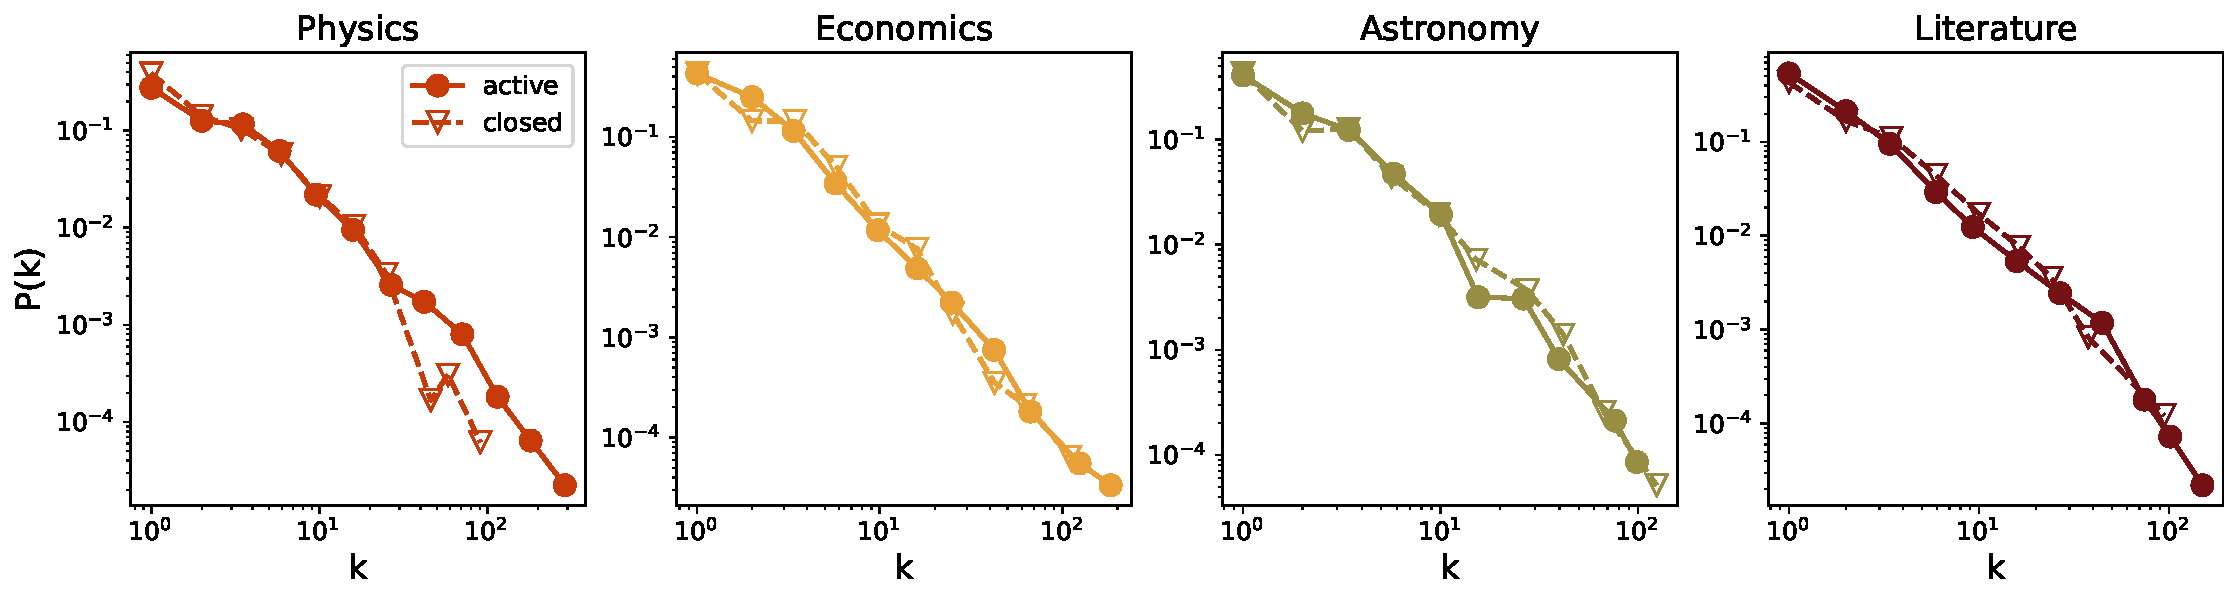
\includegraphics[width=\linewidth]{figures/stackexchange/degree_distribution_fullnet.pdf}
 	\caption{Degree distribution.}
 	\label{fig:fullnetdeg}
 \end{figure}
 
If we take look into \textbf{neighbor degree} dependece on the node degree $k_{nn}(k)$, figure \ref{fig:fullneighdeg} we find that there are structural differences between networks formed in the active and closed communities. On average $k$-degree users in active communities have neighbors with larger degree than it is case in closed communities. The results are consistent for Physics, Economics and Literature. For Astronomy we find different behavior, where the $k_{nn}(k)$ distributions of closed communities are on the top of distributions of the active one. 

\begin{figure}[h]
	\centering
	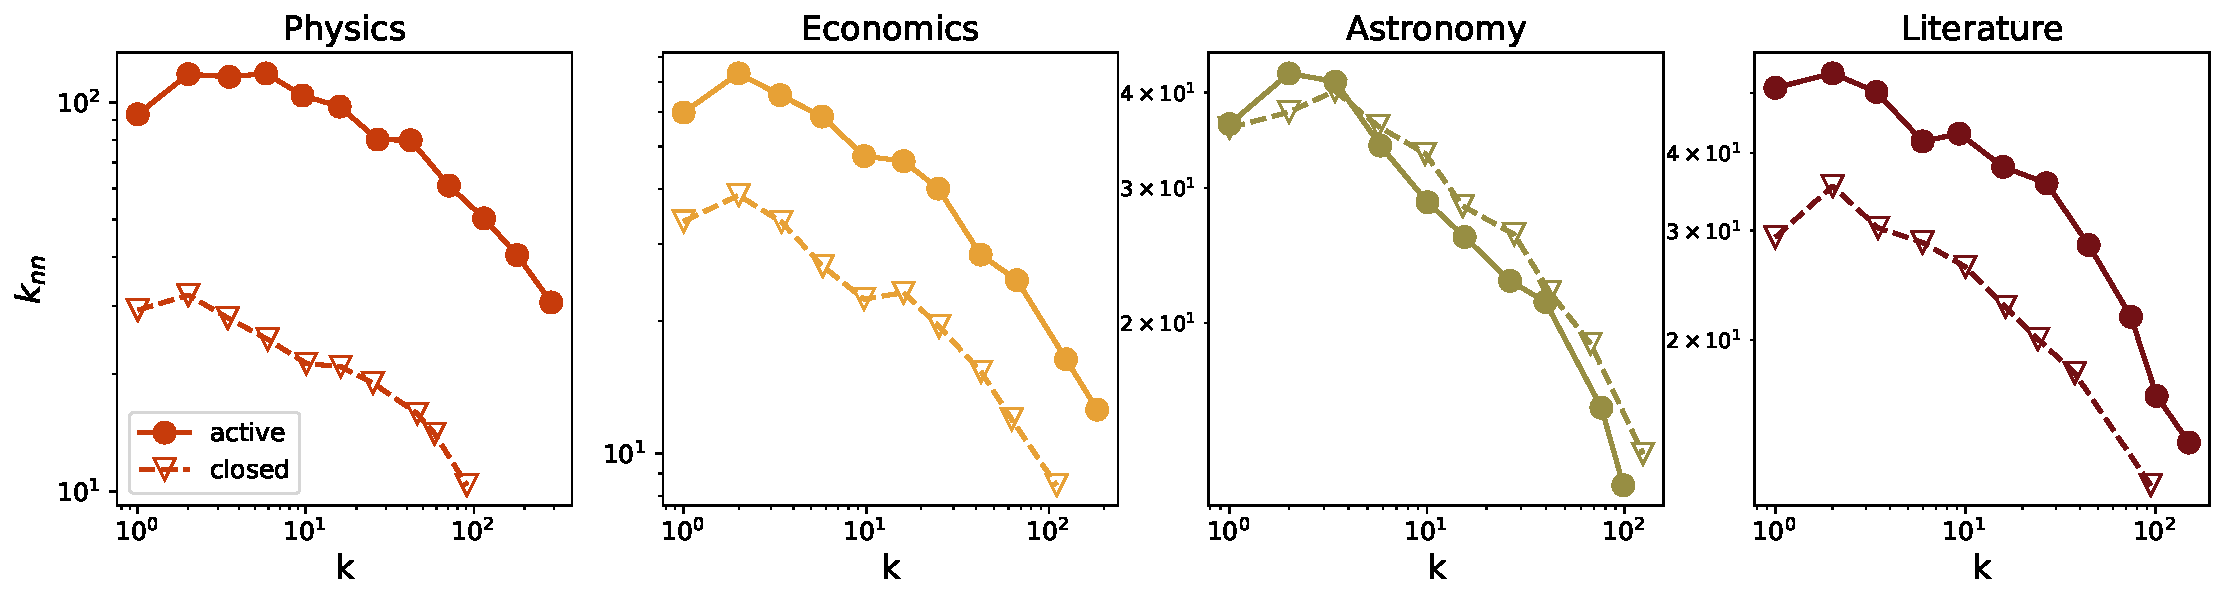
\includegraphics[width=\linewidth]{figures/stackexchange/neighdeg_fullnet.pdf}
	\caption{Neighbour degree.}
	\label{fig:fullneighdeg}
\end{figure}

The \textbf{clustering coefficient} of a node quantifies the average connectivity of between its neighbours and cohesion of its neighborhood \cite{boccaletti2006complex}. It is a probability that two neighbours of a node are also neighbours, and is calculated using the following formula:
\begin{equation}
c_{i}=\frac{e_{i}}{\frac{1}{2}k_{i}(k_{1}-1)} \ .
\label{eq:clust}
\end{equation}
Here $e_{i}$ is the number of links between neighbours of the node $i$ in a network, while $\frac{1}{2}k_{i}(k_{i}-1)$ is the maximal possible number of links determined by the node degree $k_{i}$. The clustering coefficient of network $C$ is the value of clustering averaged over all nodes. Study on dynamics of social group growth shows that that links between one's friends that are members of a social group increase the probability that that individual will join the social group \cite{backstrom2006group}. Furthermore, successful social diffusion  typically occur in networks with high value of clustering coefficient \cite{centola2007cascade}. These results suggest that high local cohesion should be a characteristic of sustainable communities. The dependence of the clustering coefficient on the node degree is shown on figure \ref{fig:fullclustering}. As expected we find that active communities are more clustered.

\begin{figure}[h]
	\centering
	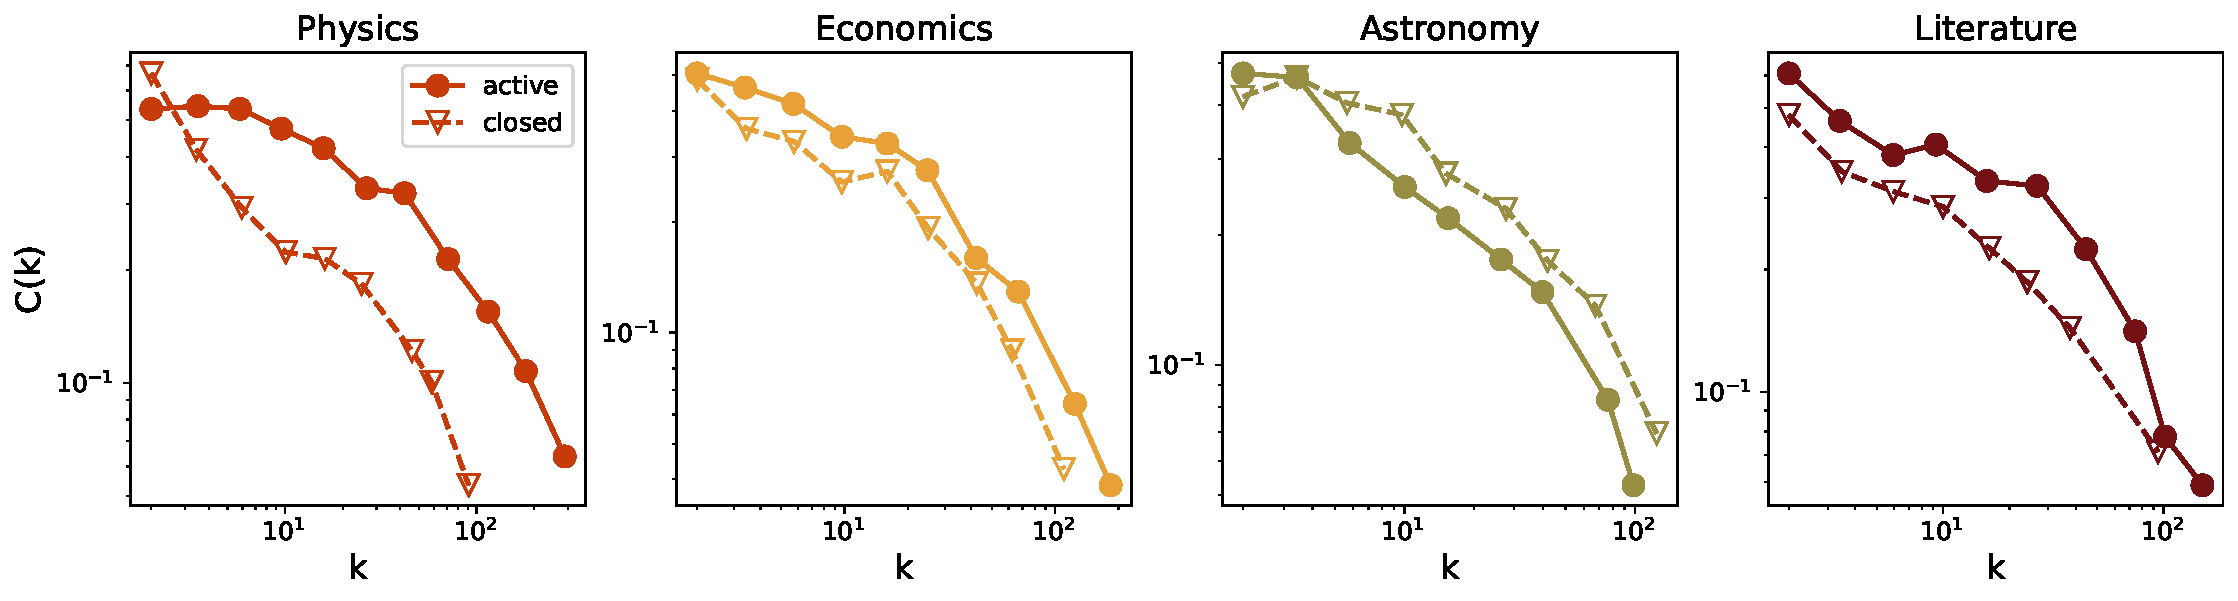
\includegraphics[width=\linewidth]{figures/stackexchange/clustering_fullnet.pdf}
	\caption{Clustering coefficient.}
	\label{fig:fullclustering}
\end{figure}

Instead of creating a static network from the data in the first 180 days of community life, we study how network snapshots evolve. At each time step $t$, we create network snapshot $G(t, t+\tau)$, for time window of the length $\tau$. We fix the time window to $\tau=30$ days and slide it by $t=1$ day through time. Discussion of how the length of the sliding window influences the results is given in appendix A. Sliding the time window by one day, we can capture changes in the network structure daily, as two 30 days consecutive networks overlap significantly. 

Here we investigate how clustering coefficient in a SE community is changing with time by calculating its value for all network snapshots. We compare the behavior of clustering for active and closed communities on the same topic in order to better understand how cohesion of these communities is changing over time. Figure \ref{fig:clustering} shows the evolution of mean clustering coefficient for all eight communities. All communities that are still alive are clustered, with the value of mean clustering coefficient higher than 0.1. Physics, the only launched community, has the value of clustering coefficient above 0.2 for the first 180 days.

During larger part of the observed period, the clustering coefficient of an active community is higher compared to the clustering coefficient of its closed pair. If we compare active communities with their closed counterpart, the closed communities have higher value of the mean clustering coefficient in the early phase while later communities that are still active have higher values of clustering coefficient. These results suggest that all communities have relatively high local cohesiveness, and that lower values of clustering coefficient in the later phase of community life may be an indicator of its decline. 

\begin{figure}
	\centering
	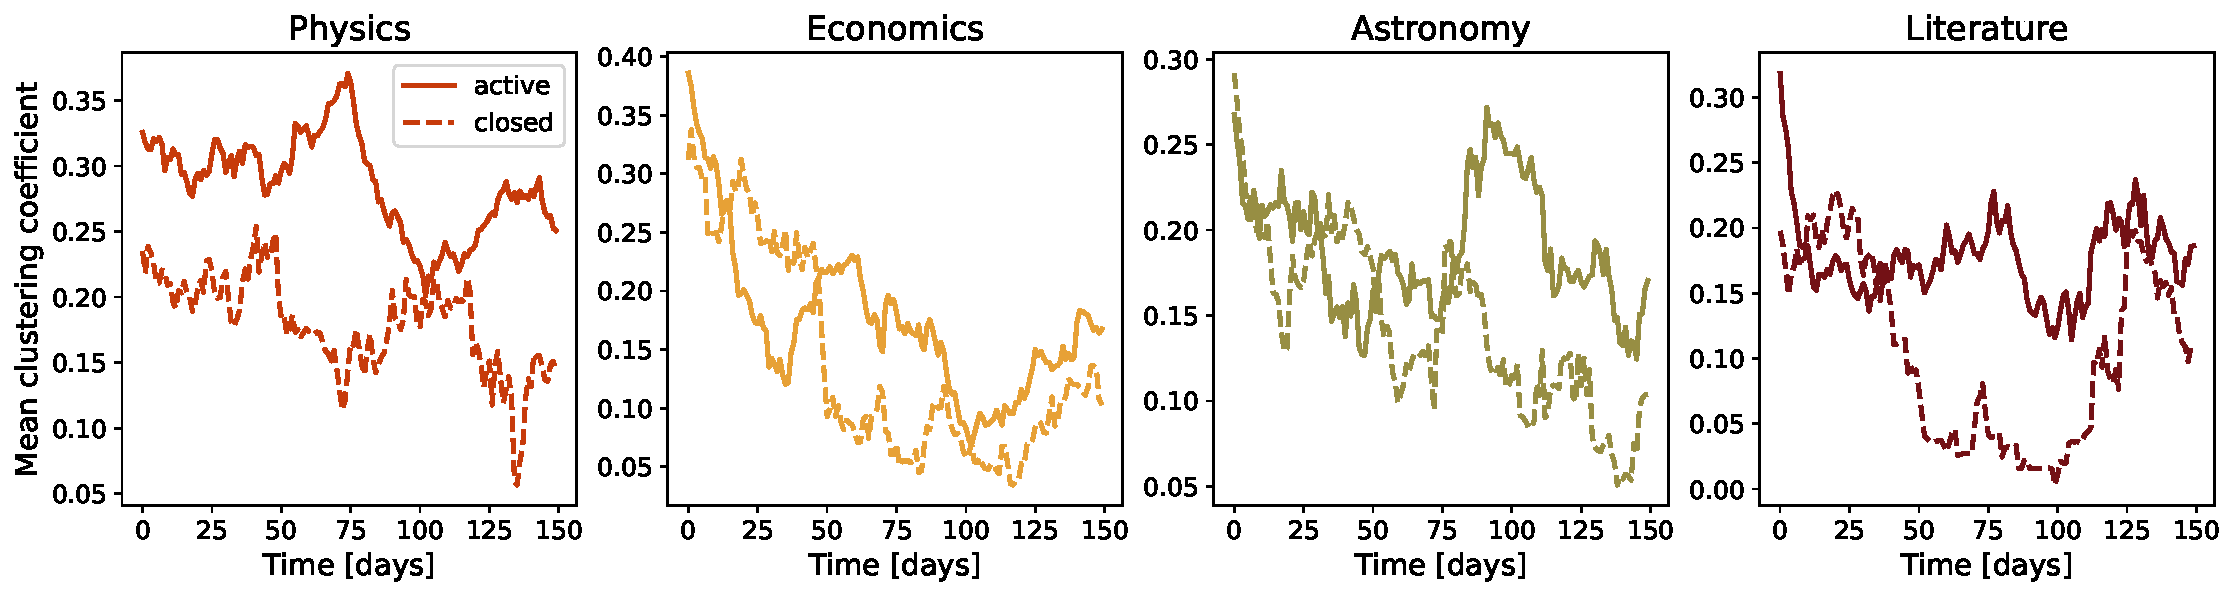
\includegraphics[width=\linewidth]{figures/stackexchange/clustering.pdf}%Figures/figures_SE/Fig3.pdf}
	\caption{Mean clustering coefficient.}
	\label{fig:clustering}
\end{figure}

\section{Core-periphery structure}

Previous research on Stack Exchange communities have attempted to explain how different types of users interact. In Question-Answer communities are expected popular and casual users \cite{santos2019activity, santos2019self}. Popular users generate the majority of interactions in the system, they are experts in community and take care on answering questions and engage the discussions through comments. As popular users they considered the $10 \%$ of the most active users, and showed that popular users are highly connected not only among themselves but also with casual users.

We tested this theory on all eight communities. We focused on 30 days sub-networks and showed how the number of links per node among popular users and between popular and casual users, evolve over time, figure \ref{fig:pop_cas_users}. We also compare active and closed communities of the same topic, so links per nodes in active sites are larger than in closed communities.

\begin{figure}[h!]
	\centering
	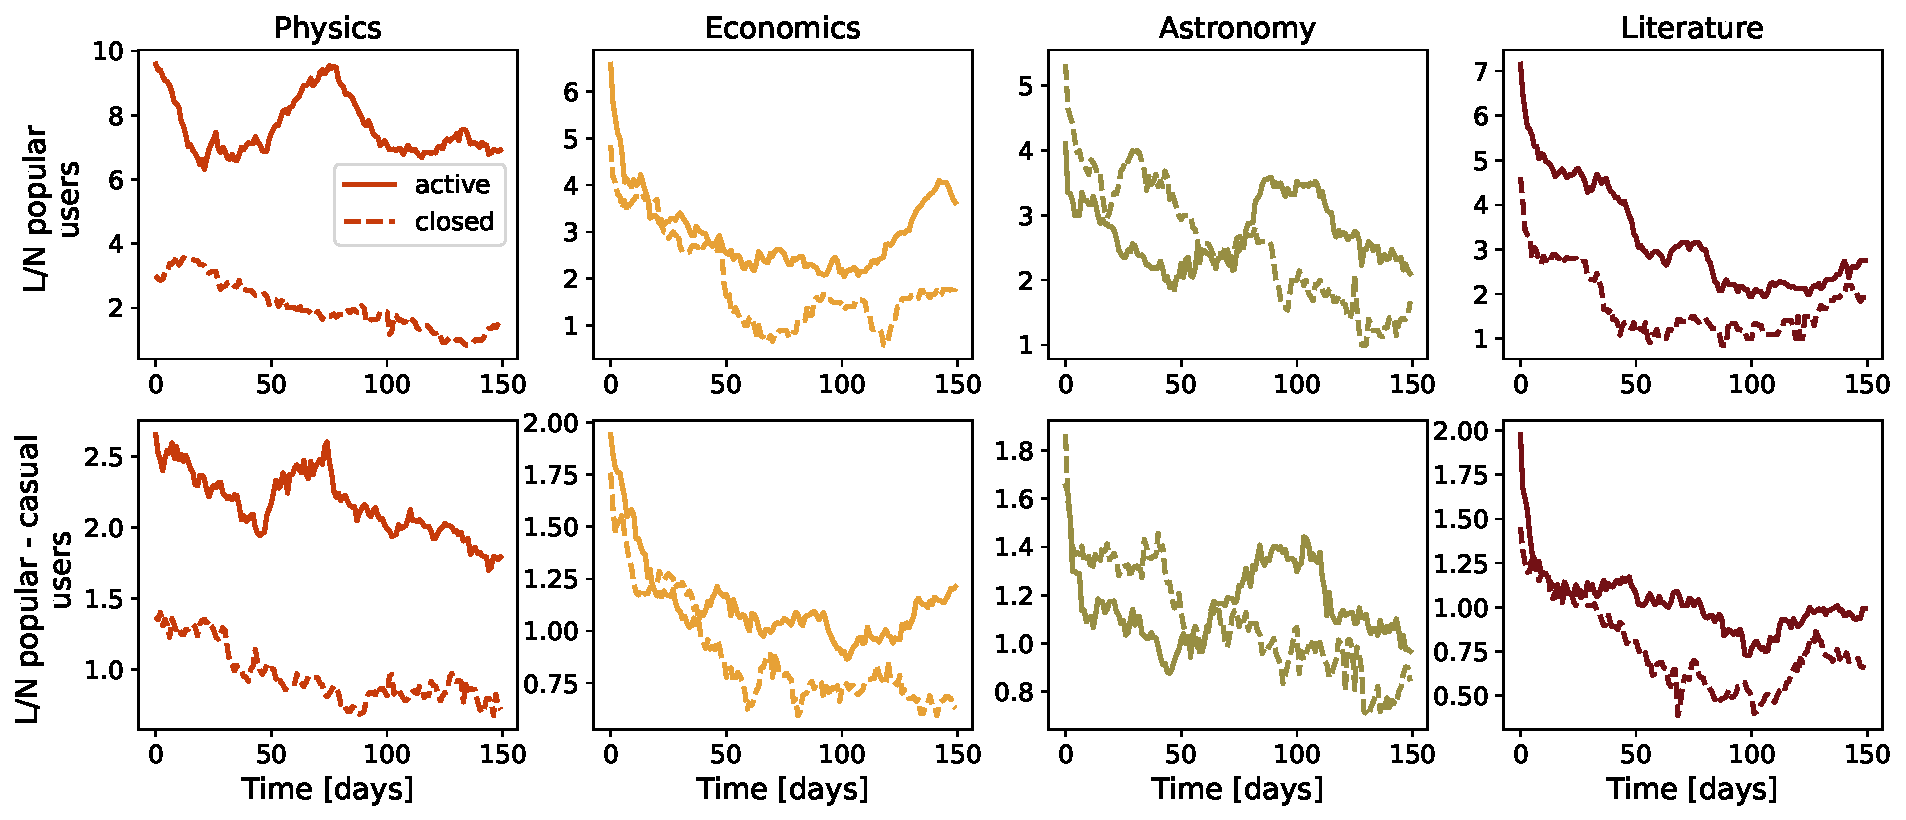
\includegraphics[width=\linewidth]{figures/stackexchange/popular_casual_users.pdf}
	\caption{Links per node among popular users (top 10\% of users) and between popular and casual users (everyone but popular users).}
	\label{fig:pop_cas_users}
\end{figure} 

Although, we find the difference between active and closed communities, the split according to $10\%$  most active users does not guaranty that all popular users will be considered. Furthermore, the smaller group of frequently active users is similar to the core users in core-periphery structure. This is why we are going to detect the core of the each 30day network. By this, separation is based on the network structure, and is more consistent, as using algorithmic approach we optimize the connectivity inside the core, periphery and among them. Core-periphery structure has core that is densely connected group of nodes, while the periphery has low density \cite{fortunato2010community, gallagher2020clarified}. 

We use Stochastic Block Model (SBM) to infer the core-periphery structure of each 30 days network snapshot and analyses how core structure evolve over time.  The  SBM algorithm is adapted for inferring the core-periphery structure, \cite{gallagher2020clarified}. For each 30 days network we run the sample of 50 iterations and choose the model parameters according to minimum description length. As stochastic models start from the random configuration, they can converge to different states, so we analyzed the stability of the inferred structures. More details are given in the appendix. We found that obtained structures differ, but minimum description length does not fluctuate too much. Also, different similarity measures between inferred core configurations take values higher than 0.9, indicating that core structure is stable. 

Number of users in core of active communities is higher than in closed communities, top panel on figure \ref{fig:core_size}. On the other hand we do not find strong difference between the fraction of core users in the closed and active communities. Furthermore, the fraction of users in core differ from the $10\%$, and it is constantly changing, bottom panel \ref{fig:core_size}. 

\begin{figure}[h!]
	\centering
	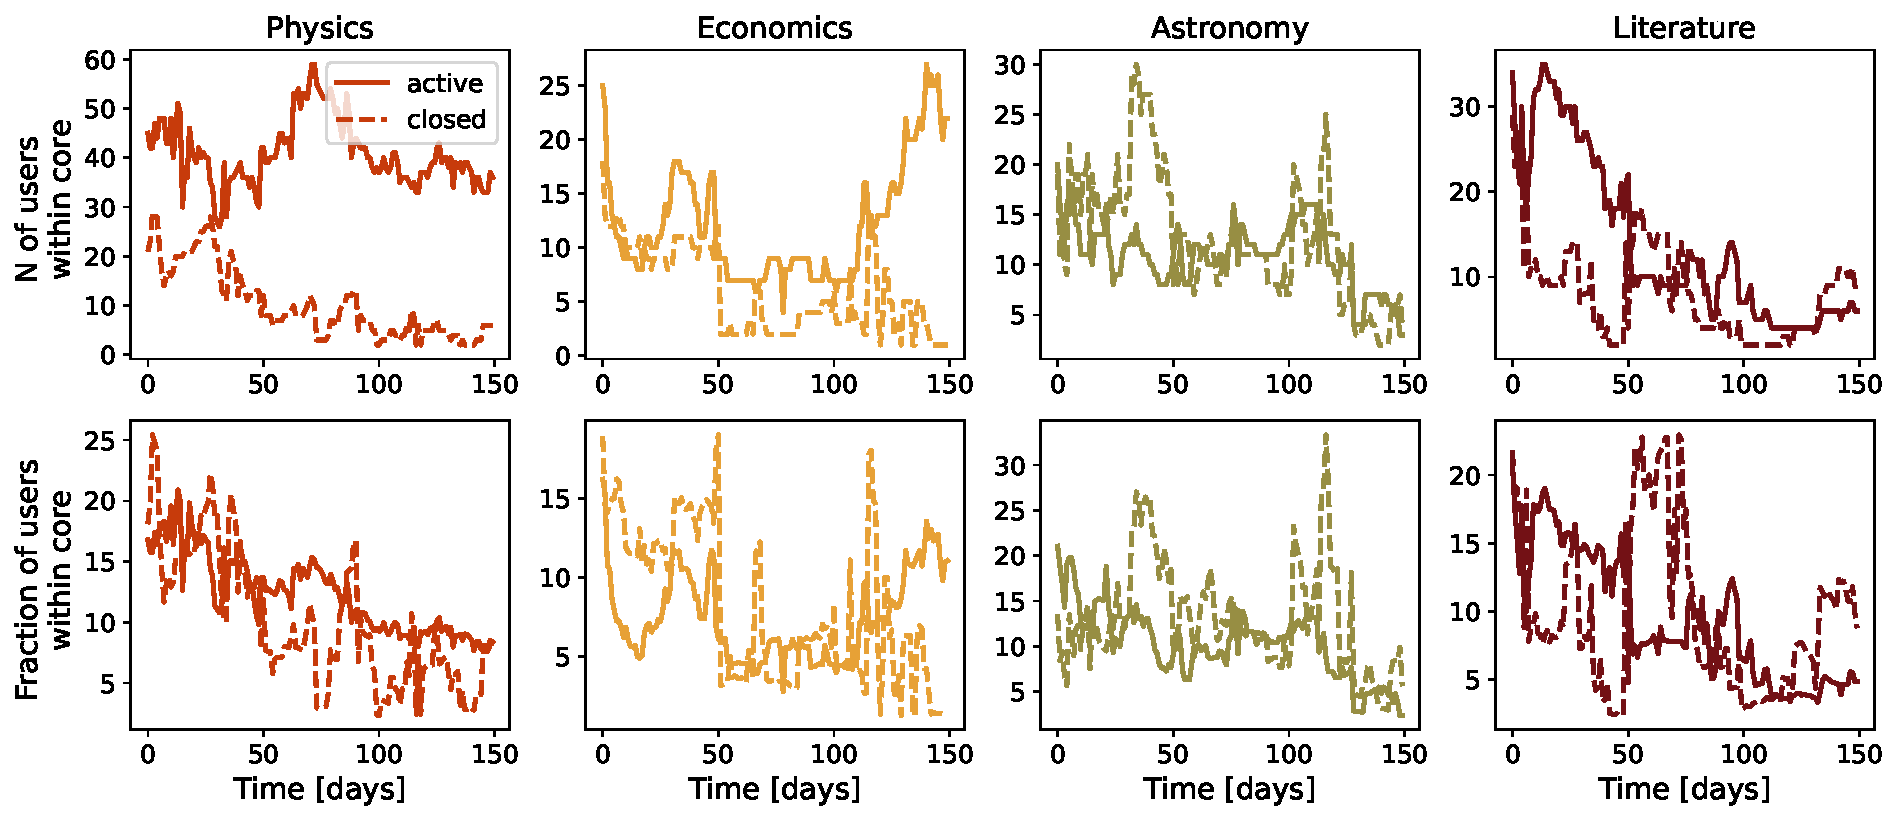
\includegraphics[width=\linewidth]{figures/stackexchange/core_users.pdf}
	\caption{Just for reference size of the core (top) and fraction of users in core (bottom). Solid lines - active sites; dashed lines - closed sites.}
	\label{fig:core_size}
\end{figure}

The number of users is constantly changing. To quantify, the stability of the core structure we compute the Jaccard's coefficient between core users in networks at time points $t_1$ and $t_2$. The Jaccard coefficient range from 0 to 1, so the larger values of Jaccard index indicate the more similar cores. 
The highest values are found around diagonal elements where we compare networks closer in time, see figure \ref{fig:jaccard_hm}. The core membership is changing over time, and it is more frequent in the closed communities. 

\begin{figure}[h!]
	\centering
	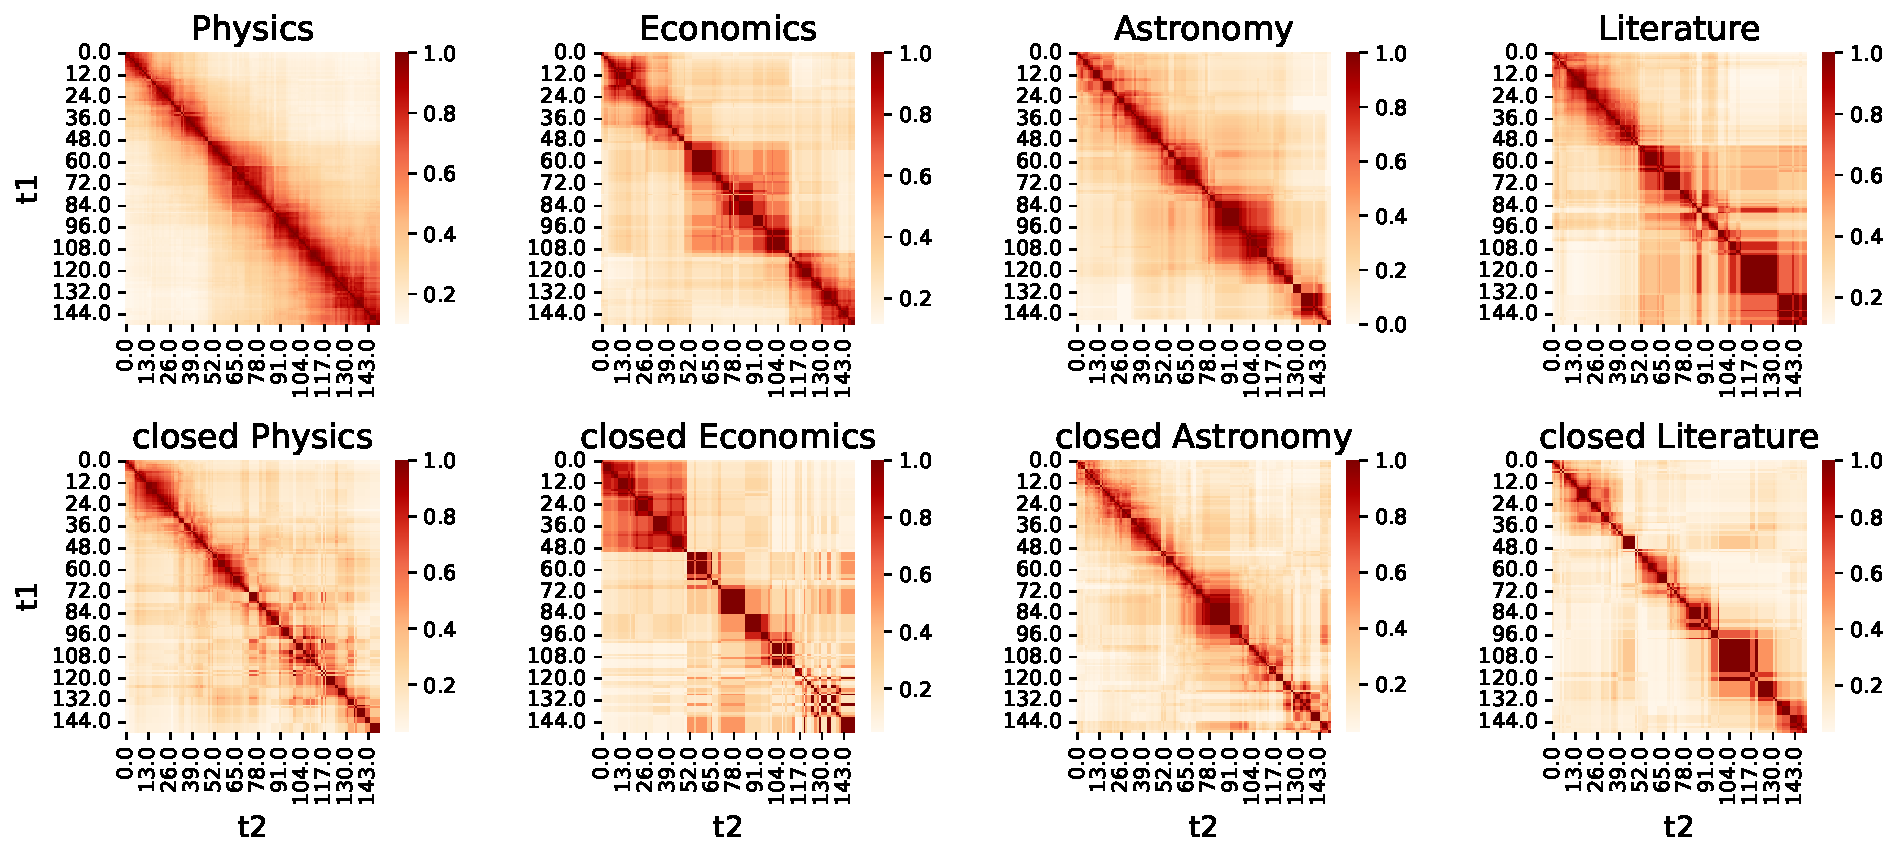
\includegraphics[width=\linewidth]{figures/stackexchange/jaccard_heatmap.pdf}
	\caption{Jaccard index between core users in  sub-networks at time points $t1$ and $t2$}
	\label{fig:jaccard_hm}
\end{figure}  

The average Jaccard index between cores in networks separated by time interval $t_i-t_j$ with the standard deviation confidence interval are shown in figure \ref{fig:jaccard_mean}. The Jaccard index decreases with relative time difference between networks faster in closed communities. The relatively high overlap between distant networks confirms that active networks have more stable core. 

\begin{figure}[h!]
	\centering
	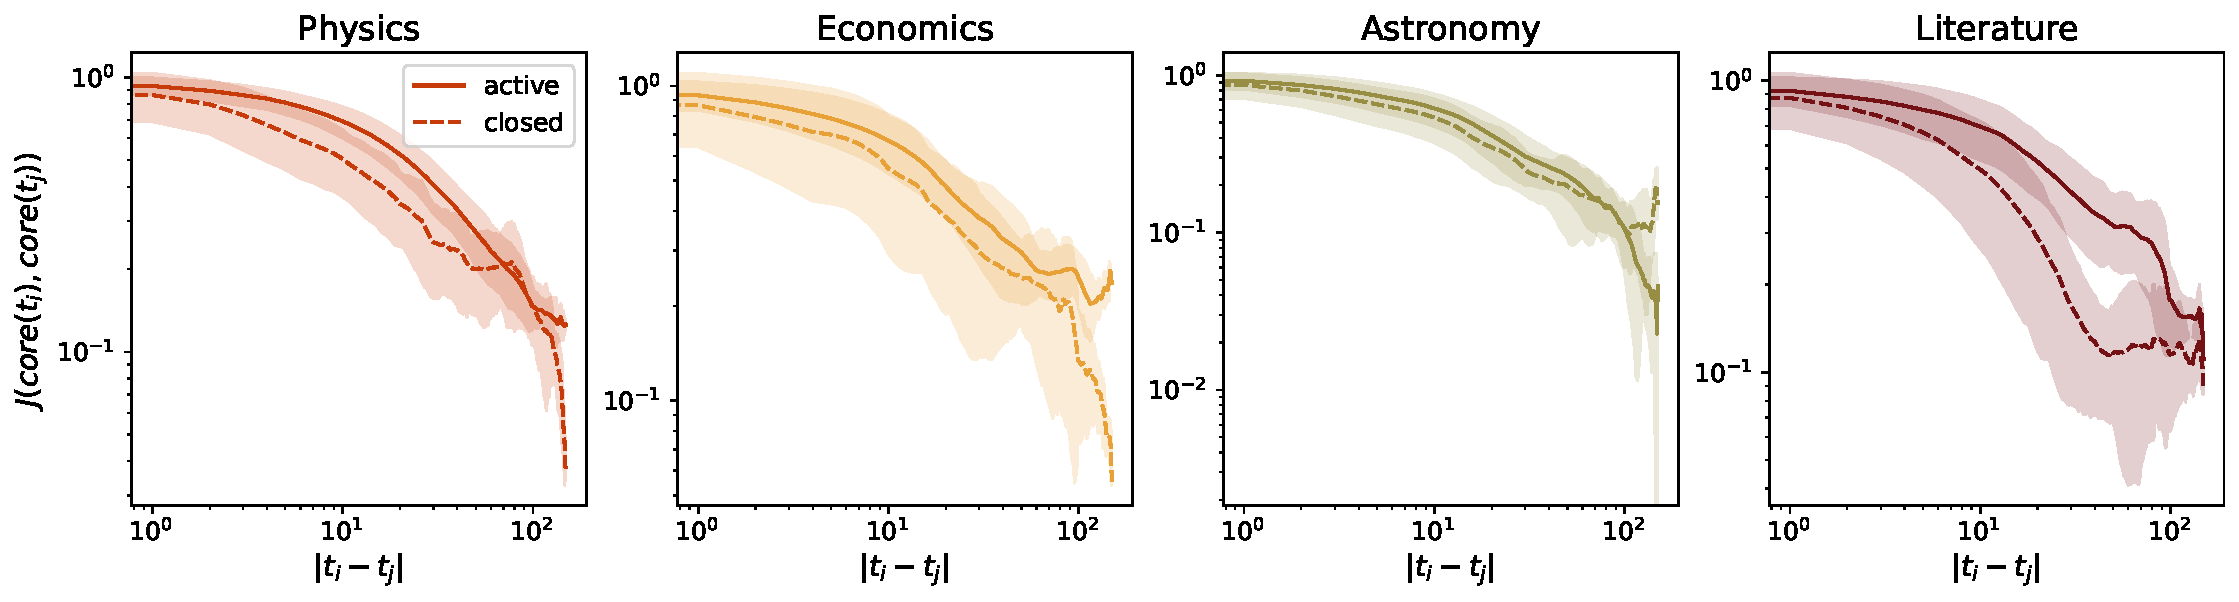
\includegraphics[width=\linewidth]{figures/stackexchange/jaccard.pdf}
	\caption{Jaccard index between core users in 30days sub-networks for all possible pairs of 30 days sub-networks separated by time interval $|t_i - t_j|$}
	\label{fig:jaccard_mean}
\end{figure}

Finally, we examine how the connectivity of the users in the core and between core and periphery evolve over time. On figure we show the $L/N$ in the core, that is proportional to the average degree of the network $2L/N$. The Physics community has more than twice larger connectivity than closed Theoretical Physics. For Literature we also find higher connectivity, but at the end of observation period the values become, the connectivity in active site drops and becomes similar as in closed one. For Economics and Astronomy the difference between active and closed site is not so clear. At the beginning of the period for the sites on economic topic, connectivity is similar, After 50 days of community life, connectivity in active communities is starting to rise, while in the case of closed economics it is dropping. For Astronomy, the connectivity is higher in closed communities, in the first 50 days, After this, period we find the sudden rise in the connectivity of active astronomy, but again it is dropping and becomes comparable to the connectivity values in closed site. The similar conclusions can be drawn for the connectivity between core and periphery. The largest difference between active and closed site is observed for Physics.  When it comes to active communities that are still in the beta phase, they either have the same core-periphery connectivity as their closed counter part, or as in the case of Astronomy, their periphery is weaker connected to the core during the first 50 days of their life, see Fig. \ref{fig:links_per_node}. 

\begin{figure}[h]
	\centering
	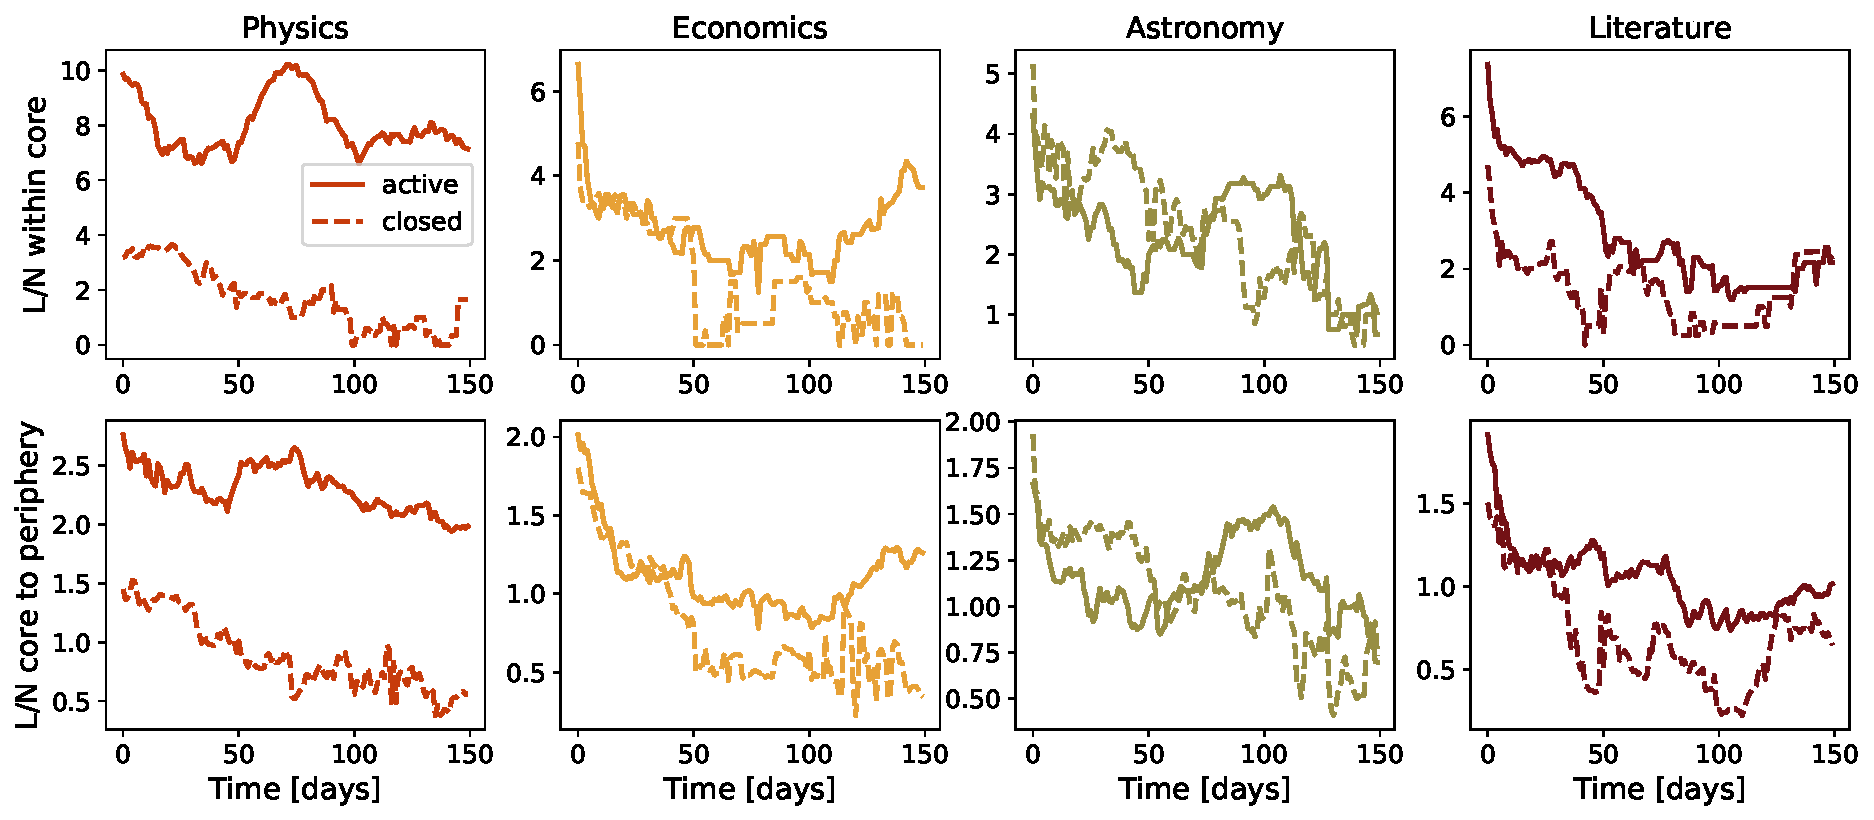
\includegraphics[width=\linewidth]{figures/stackexchange/core_connectivity.pdf}
	\caption{Links per node in core and links per node between core and periphery.}
	\label{fig:links_per_node}
\end{figure}

\section{Dynamical Reputation model}

We further explore the difference between active and closed communities through the dynamical reputation model. With this model we calculate the reputation of each user in the community. The reputation is directly connected with the collective trust in the network. 

\begin{figure}[h]
	\centering
	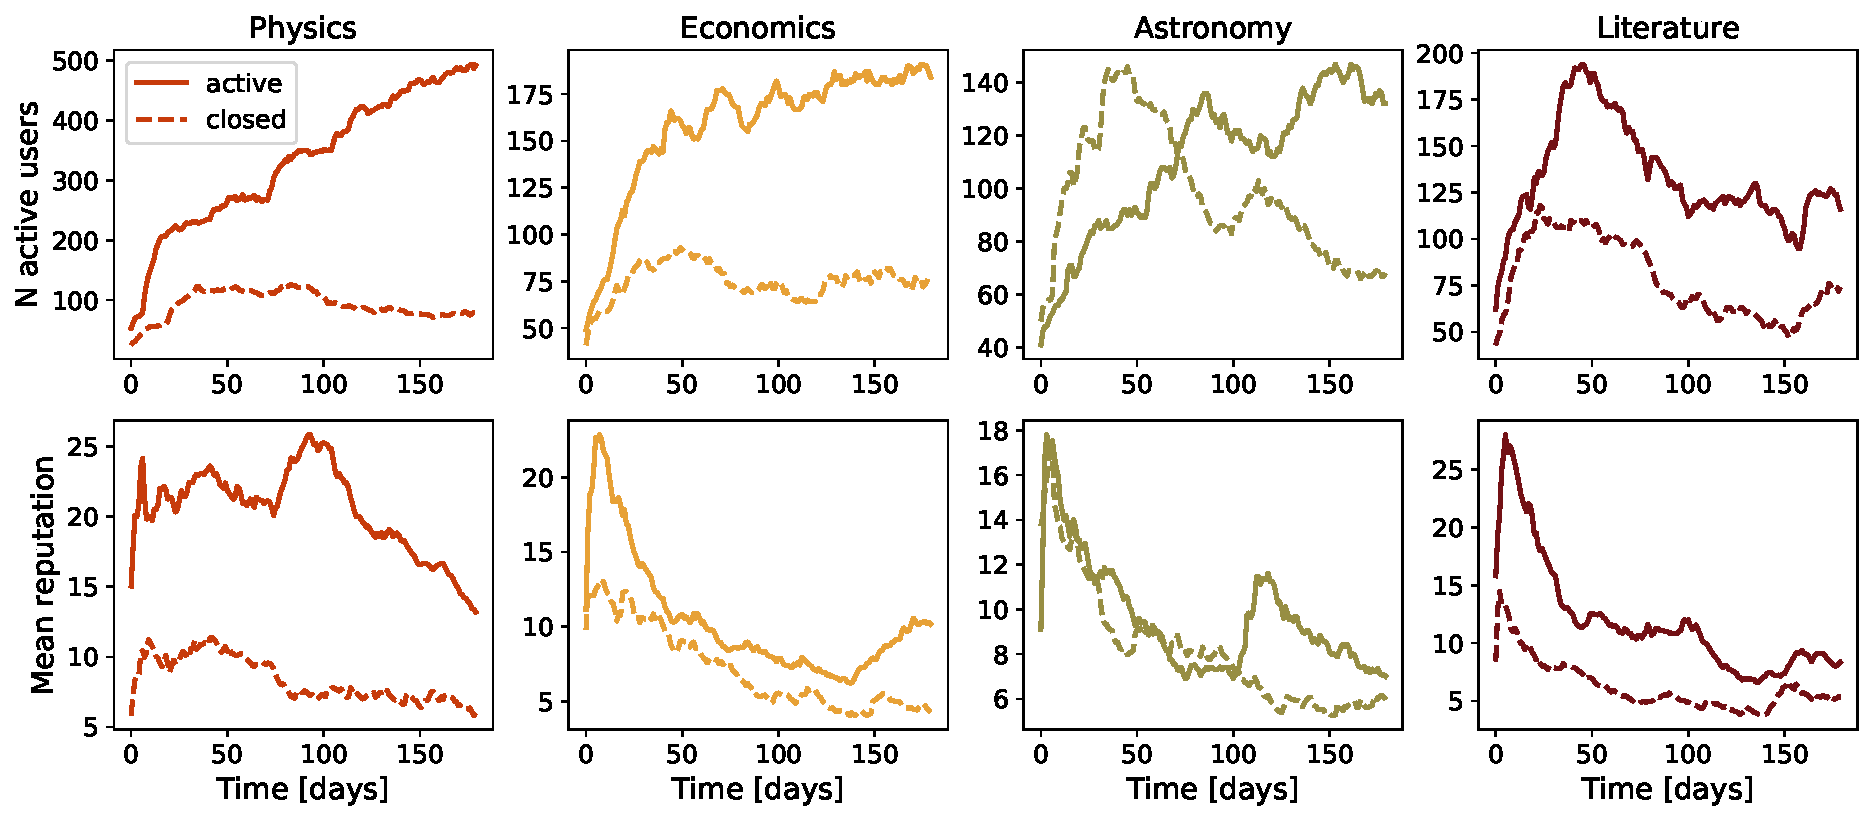
\includegraphics[width=\linewidth]{figures/stackexchange/reputation.pdf}
	\caption{Dynamic Reputation on the four pairs of Stack Exchange websites: Astronomy, Literature, Economics,  Physics and Theoretical Physics.}
	\label{fig:dr6panel}
\end{figure}



Dynamical reputation model, introduced in section \ref{sec:met_dibrm} has three parameters. We explored different parameter combination, to find the set of parameters the most suitable for given system of Stack Exchange communities. First of all, the basic reputation is set to $I_{bn}=1$. The cumulative factor is $\alpha=2$, as we want to emphasize the frequent interactions. The parameter $\beta$ controls the reputation decay due to user inactivity. After last activity, for some period user has positive reputation still making impact on the other users. We optimized the the number of users with reputation larger than $1$ according to the number of users in the 30 days network, so parameter $\beta=0.96$. The discussion about the parameters choice is in appendix. 

With selected model parameters, we calculated the the reputation of each user. If user has the reputation larger than $1$, it is considered as active, but when the reputation drops below this threshold means that user has not be active long enough and it is not give valuable contribution for the community. The number of active users and their mean reputation for different SE sites are shown in figure \ref{fig:dr6panel}. 

From network properties we found that active communities are more cohesive and have more stable core. Furthermore, we focus our analysis on the dynamical reputation of the core users. The figure \ref{fig:dr_core} shows the evolution of mean user reputation within core. Active communities have larger reputation than closed counterpart. As it is previously suggested, the largest difference is found for Physics community. For other communities, difference is not so striking, still on average the core of active communities has larger reputation than core of closed communities. 

\begin{figure}[h]
	\centering
	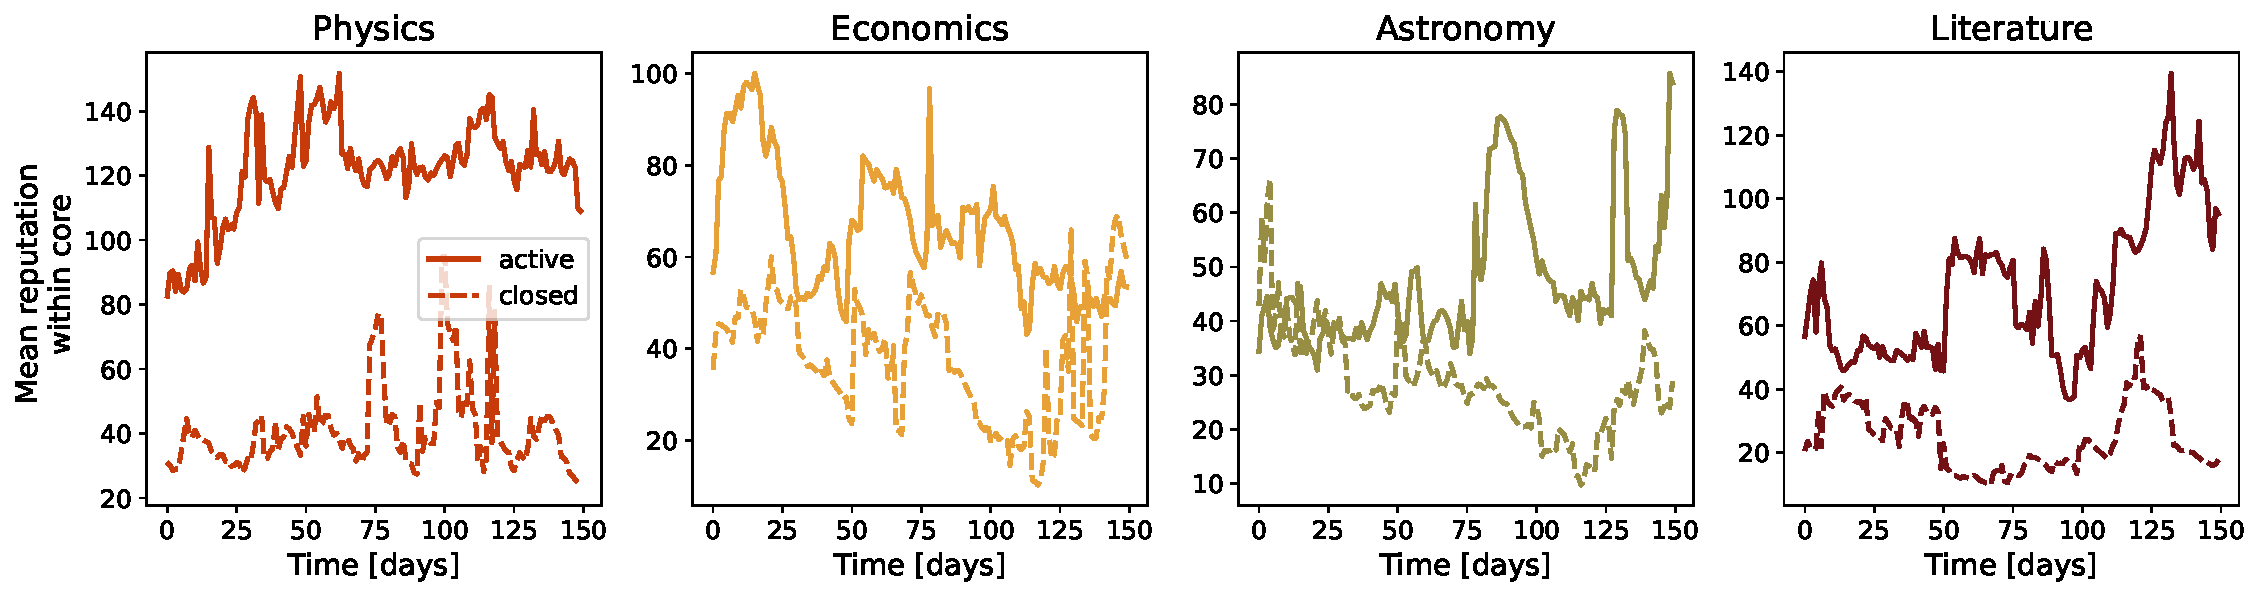
\includegraphics[width=\linewidth]{figures/stackexchange/core_reputation.pdf}
	\caption{Dynamical reputation within core.}
	\label{fig:dr_core}
\end{figure}

In the core of the network are very active users and we expect higher dynamical reputation in the core in comparison to the total reputation of users belonging to periphery. The ratio between core and periphery in Physics is always higher than in Theortical Physics. Similar conclusions are observed for literature. For the early days of Economics, we find different pattern, the core-periphery reputation ratio is larger for closed Economics, but later this changes in the favor of active Economics. Astronomy shows different behavior where the closed community where dominantly, closed astronomy had larger core-periphery reputation ratio. 

\begin{figure}[h!]
	\centering
	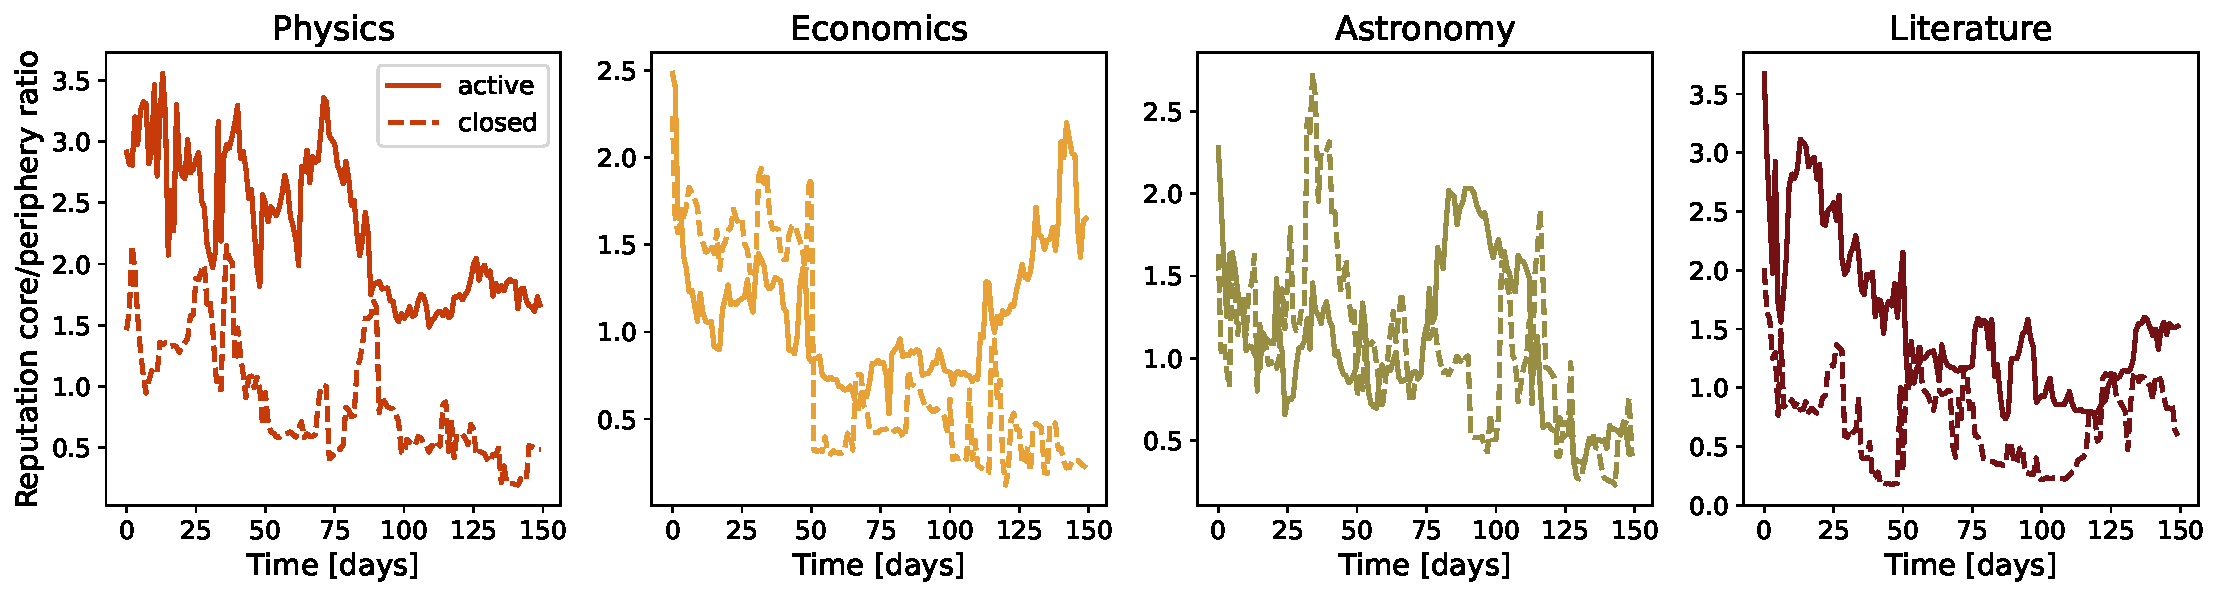
\includegraphics[width=\linewidth]{figures/stackexchange/core_per_ratio_reputation.pdf}
	\caption{Ratio between the total reputation within network core and periphery. Solid lines active communities, dashed lines closed communities.}
	\label{fig:dr_core_per}
\end{figure}

The distribution of the dynamical reputation of SE communities are skewed. To better express the difference between distribution reputation we calculated the Gini coefficient. This measure quantifies the inequality among users reputation. The gini coefficient is calculated based on reputation values for each day, see figure \ref{fig:dynrep-gini}. The gini coefficient is larger than $0.5$, in the first 180 days. Also, in the active communities showed more reputation inequality and dynamical reputation has larger variation. 

\begin{figure}[h]
	\centering
	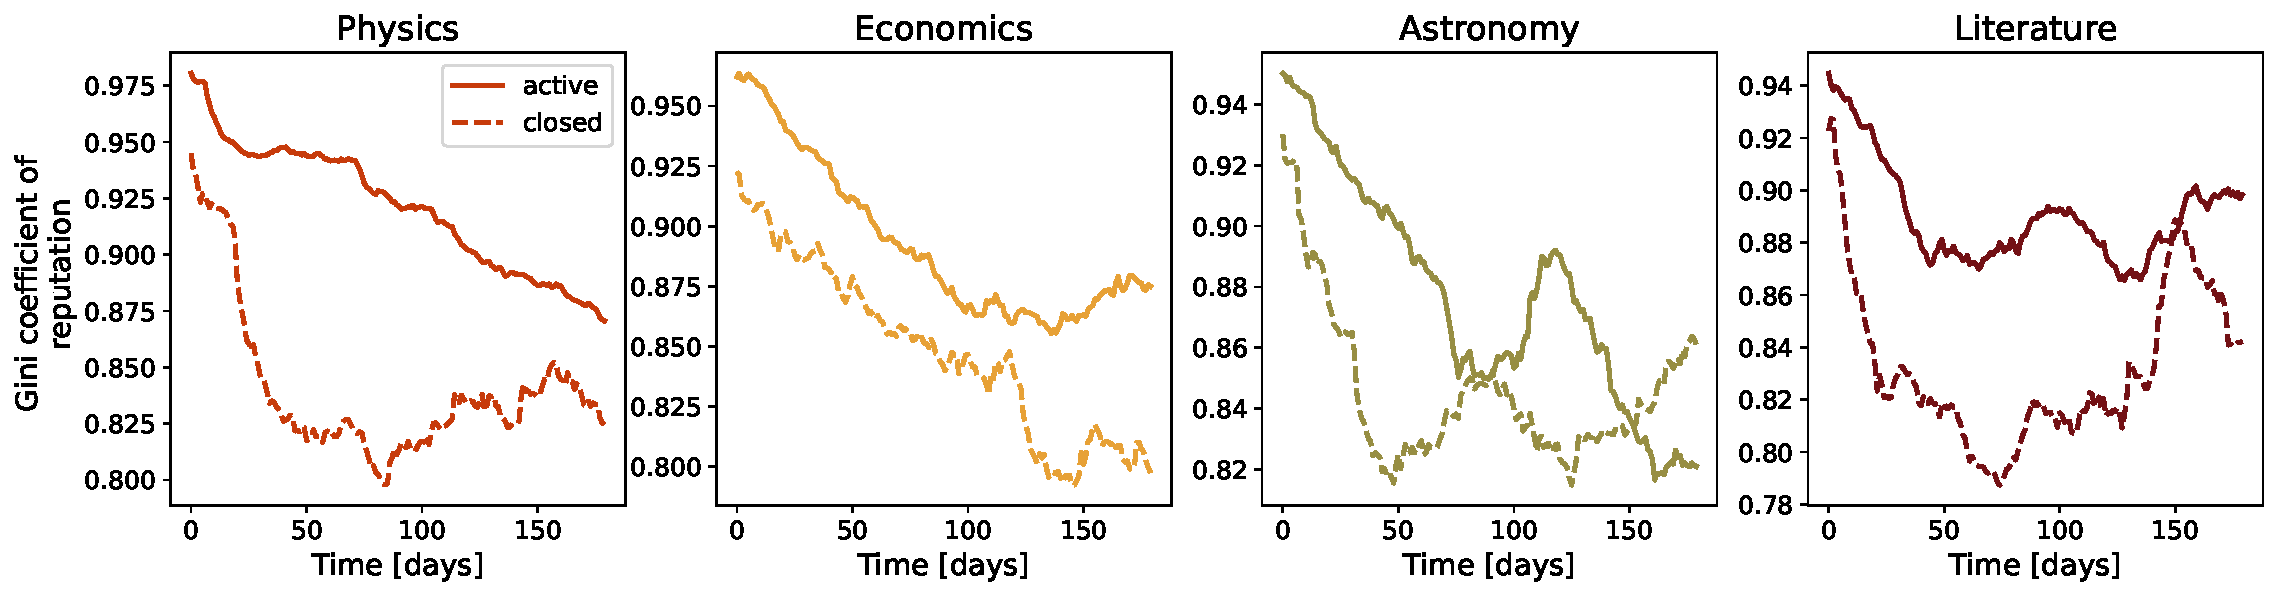
\includegraphics[width=1\linewidth]{figures/stackexchange/gini.pdf}
	\caption{Gini index of dynamic reputation within population}
	\label{fig:dynrep-gini}
\end{figure} 

Further, we investigate how properties of user interaction network are correlated with the reputation of user. For example we can use measure the assortativity coefficient among connected users in the network. For each 30 days user interaction network, we calculate the reputation assortativity, using reputation value observed in the last day of the time window in which the network is constructed. With this measure we quantify weather users tend to connect with users with similar reputation or not. Figure \ref{fig:dyn_rep_assort} shows results where for each SE community we compare the active and closed site. In all communities reputation assortativity has small values, not larger than $|0.3|$. In active communities this is mostly negative measure showing expected user behavior, popular users, who often have the high dynamical reputation interact with users with low dynamical reputation. Astronomy is outlier again, during first 100 days active community had positive reputation assortativity and after this period, it started to behave similar as other active communities. 

\begin{figure}[h]
	\centering
	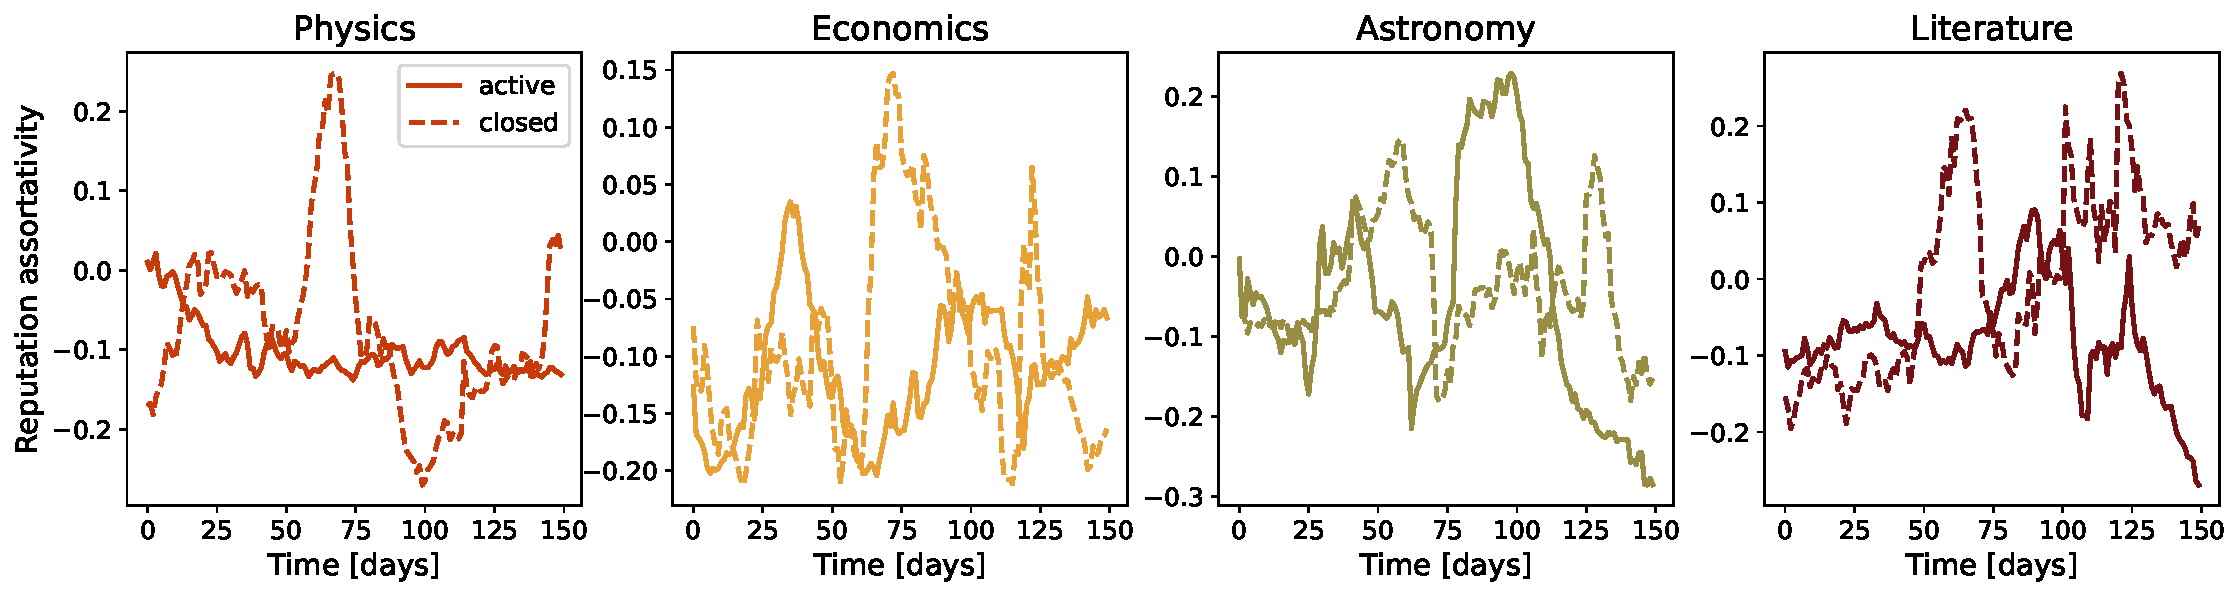
\includegraphics[width=1\linewidth]{figures/stackexchange/reputation_assortativity.pdf}
	\caption{Dynamic Reputation assortativity in the network of interactions (questions, answers, comments, unweighted, undirected network). Solid lines - active sites; dashed lines - closed sites.}
	\label{fig:dyn_rep_assort}
\end{figure}

We continue to investigate whether the user's reputation correlates with typical network centrality measures calculated at user's node in the interaction network. As previously, we compare node's centrality in the 30 day network with the node's dynamic reputation on the last day of the period, repeat the process every day for the first six months. 

Correlation coefficient between dynamic reputation and degree in the network is very high, as expected, as most of the interactions that contributed to user's reputation are also present as links in the network. We show these results in Fig.~\ref{fig:dyn_rep_centrality}(top). However, we again see the distinction between active and closed communities where this correlation is higher in active communities, except in the first month of sliding windows. Astronomy is an exception here as well as we see that the correlations were similar in both closed and still active sites throughout observed period. 


In the bottom panels of Fig.~\ref{fig:dyn_rep_centrality} we present correlation coefficients of dynamic reputation and user's betweenness centrality in the interaction network. These corrlations are also high and most of the time higher in the later networks of active than closed communities. This is particularly interesting due to global nature of betweenness centrality measure and less obvious relation of it to user's dynamic reputation.

\begin{figure}[h!]
	\centering
	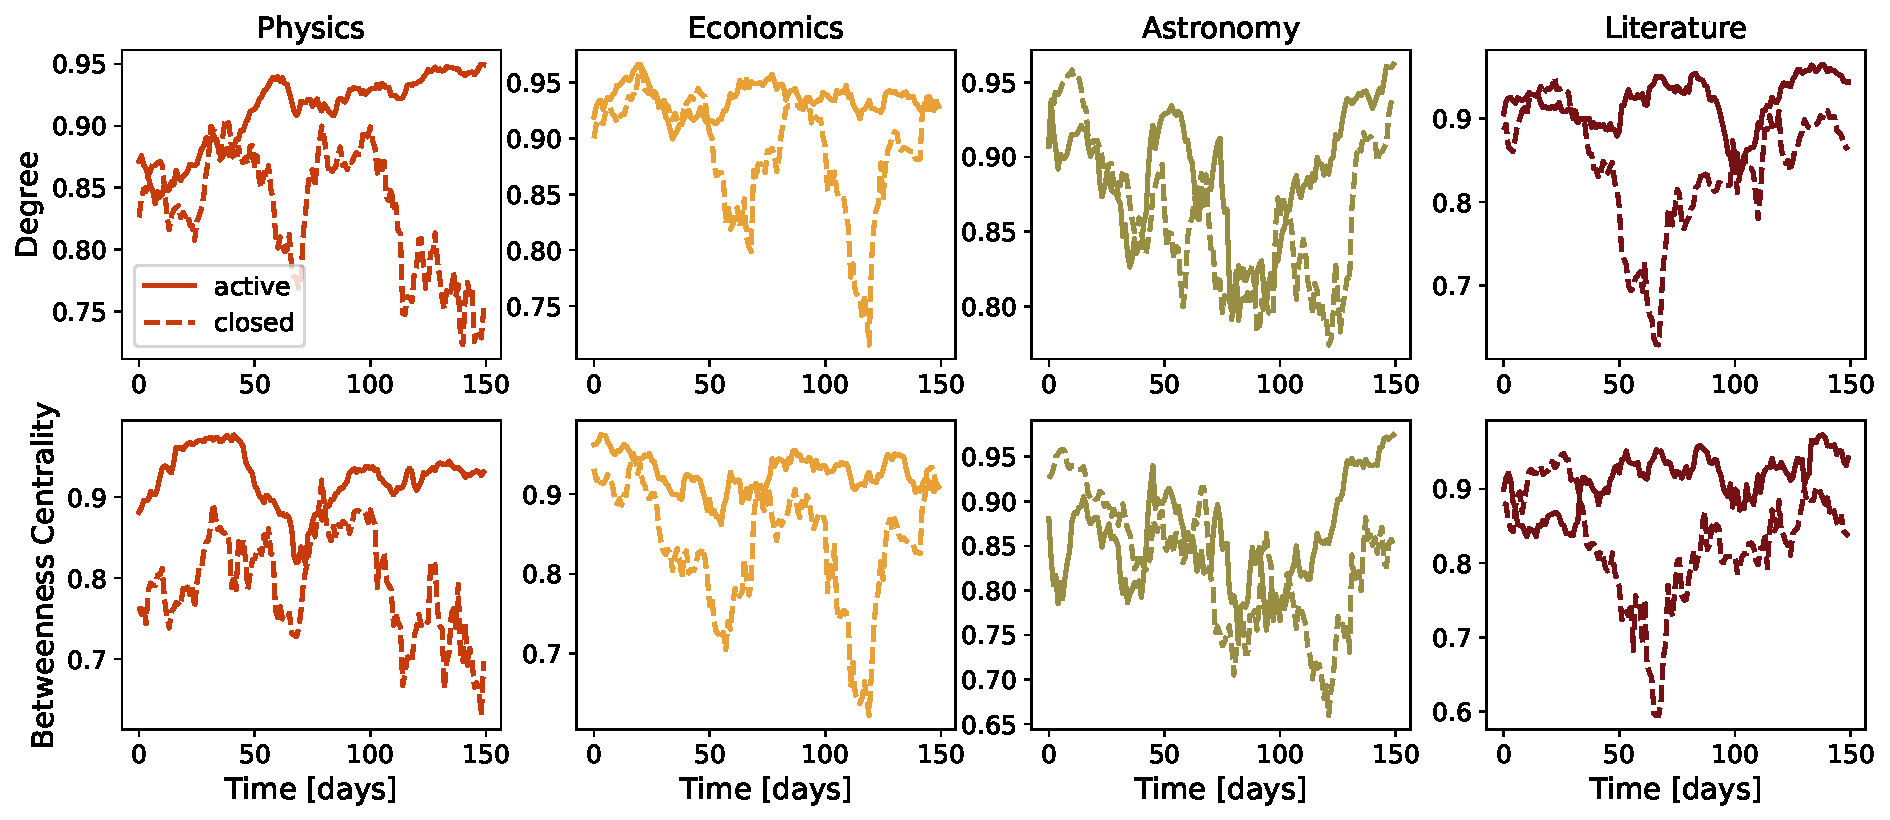
\includegraphics[width=\linewidth]{figures/stackexchange/correlations.pdf}
	\caption{Coefficient of correlation between users' Dynamic Reputation and users' network degree (top) and users's betweenness centrality (bottom). Solid lines - active sites; dashed lines - closed sites.}
	\label{fig:dyn_rep_centrality}
\end{figure}




